\documentclass[bibtotocnumbered, headsepline,normalheadings]{report}
\usepackage[latin1]{inputenc}
\usepackage{color}
\usepackage{booktabs}
\usepackage{multirow}
\usepackage{listings}
\lstset{breaklines=true,showstringspaces=false,numbers=left,frame=single,prebreak=\mbox{$\hookleftarrow$}}
\usepackage{hyperref}
\usepackage[a4paper,margin=2cm]{geometry} 
\usepackage{scrpage}
\usepackage{alltt}
\usepackage{float}
\usepackage{graphicx}
\definecolor{darkblue}{rgb}{0,0,.5}
\hypersetup{pdftex=true, colorlinks=false, breaklinks=true, citecolor=darkblue, linkcolor=darkblue, menucolor=darkblue, pagecolor=darkblue, urlcolor=darkblue,
pdftitle={Universal Translator for Wireless Sensor Node Networks},
pdfauthor={Bartholom�us Dedersen, Kamil Wozniak},
bookmarks=true,
bookmarksnumbered=true,
bookmarksopen=true,
bookmarksopenlevel=2}
\pagestyle{headings}
\begin{document}

\author{ 
Bartholom�us Dedersen \\ Fachhochschule Kiel \\ bartholomaeus.dedersen@student.fh-kiel.de \and
Kamil Wozniak  \\ Fachhochschule Kiel \\ kamil.a.wozniak@student.fh-kiel.de }

\date{\today} 
\title{Universal Translator for Wireless Sensor Node Networks} 

\maketitle


\begin{abstract}
Kamil likes to write abstracts and does not deny it.
\end{abstract}

\tableofcontents \newpage

\chapter{Introduction}

Wireless Sensor Nodes \footnote{We will refer instead of the long form to the abbreviation \textsc{WSN} in the remaining documentation.}
are versatile low-power embedded systems used for monitoring sensors, measuring concentration of various chemicals, meshed communication
and a multitude of other purposes.

They were developed by the DARPA\cite{Song}. First tries to established small networked sensors can be traced back to the cold war according to
\cite{Chong}:

\begin{quote}
    ``During the Cold War, the Sound Surveillance System
    (SOSUS), a system of acoustic sensors (hydrophones) on the
    ocean bottom, was deployed at strategic locations to detect
    and track quiet Soviet submarines. Over the years, other
    more sophisticated acoustic networks have been developed
    for submarine surveillance. SOSUS is now used by the
    National Oceanographic and Atmospheric Administration
    (NOAA) for monitoring events in the ocean, e.g., seismic
    and animal activity.''
\end{quote}

Acconding to Chong et. al the research and development further increased in the year 1980 with the \textsc{Dsn}\footnote{Distributed Sensor Networks} project.
It was founded by the American military while 
``the Arpanet (predecessor of the Internet) had been operational for a number of years, with 
about 200 hosts at universities and research institutes''\cite{Chong}.
R. Kahn, one of the main responsible persons behind the early Internet and co-inventor of the TCP/IP-definitions, had special interest how networked
sensor networks would fit into the routed packed based network acconding to Chong et al..

\begin{figure}[H]
   \centering
   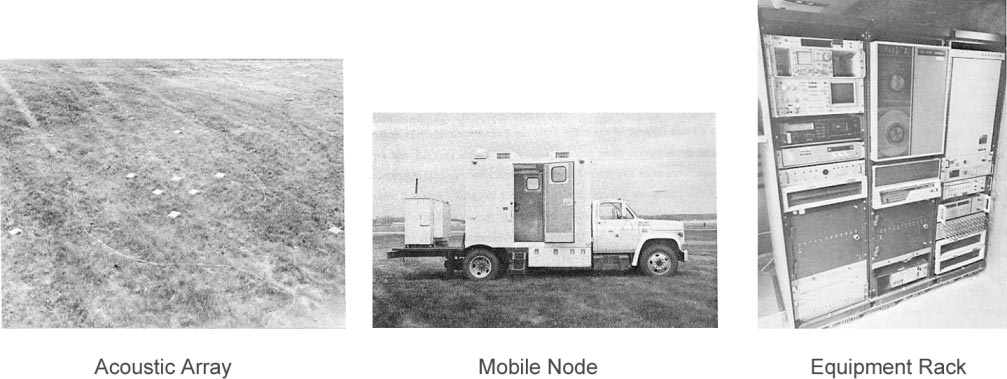
\includegraphics[width=0.8\textwidth]{pic/earlynode.png}%
   \caption{Early Sensor Nodes in 1985. Source: \cite{Chong}}
   \label{earlynode}%
\end{figure}

In~\cite{Akyildiz02wirelesssensor} various applications for military use are described. Main points are:

\begin{description}
    \item[Monitoring] How much ammunition is left in specific areas and/or assets?
    \item[Surveillance] How is the enemy advancing/retreating?
    \item[Reconnaissance] Is in a specific area an opposing force?
    \item[Targeting] Can rockets and other ammunition be assisted for targeting?
    \item[Damage Assessment] How much did our forces suffer before and after a fight?
    \item[ABC Detection] Did the opposing force utilize ABC\footnote{Atom/Nuclear, Biological and Chemical Warfare} weaponry?
\end{description}

As Akyildiz et al. described the main purpose in miliary use are 
``Wireless sensor networks can be an integral part
of military command, control, communications,
computing, intelligence, surveillance, reconnaissance
and targeting (C4ISRT) systems.
''

But rapidly civilian areas of usage were aquired. Heraklit said: ``Πόλεμος πάντων μὲν πατήρ ἐστι''\footnote{War is the father of all things} and so 
research and development about wireless sensor networks was adapted by universities and other parties.


The main points which stopped the usage in civilian areas were:

\begin{itemize}
\item battery longlivety
\item size
\item portability
\item secure communication
\item calculation speed
\item compatibility
\item lacking unified language for high-level programming
\end{itemize}

If one \textsc{WSN} is not enough for a usage scenario some form of communication between the devices is neccessary. The obvious
route is through means of wireless communication.

Different forms of wireless communication are available:

\begin{description}
\item[ZigBee] Low power but limited range through the band XXX
\item[IEEE 802.11] Popular name is \textsc{WLAN}. Mainly the 2.4 GHz band is used but in subsets like 802.11a the short-waved 5GHz band is usable.
Energy consumption is generally higher.\footnote{Regulatory standards in Germany forbid more than 150mA total power sent.}
\item[Custom radio communication] XXX Ask Dispert
\item[More] XXX Ask Koss
\end{description}

Wireless sensor nodes can be deployed and used in a multitude of means.\footnote{But not for special cases as~\cite{biederbeck}}


\chapter{Wireless Sensor Nodes}

RZB_CC28_ renesas


\chapter{Task of unifying languages}

Different communication languages exist for the big communication layers Bluetooth, ZigBee and active RFID.

In~\cite[p. 407]{Akyildiz02wirelesssensor} a hardware query language for sensors called \textsc{SQTL}\footnote{Sensor Query and Tasking Language}
is decribed. This language is, very similar to current \textsc{SQL}, supposed to give a subset of nodes querys as \textit{Which sensor does receive
something irregular(Tempererature above some treshold or detection of dangerous chemicals in environment protection} and the nodes affected 
will return their data if they match the query. Other possiblities are also described in the aforementioned article but they go into a technical
dimension as reconfiguring the possible positions of nodes and general network configuration.

Such tasks are generally meant to be solved by a versatile language. As the possibilites are just drafed and still discussed in a comitee our 
approach is a rapid iterative development cycle supported with automated tests to develop a fast solution.

To overcome this problem and establish a user-defined set of generalized commands this project was started.
The original idea was to unify various communication level layers and their corresponding dialects to 
archive easy and centralized means of sending and receiving command, i.e. one typed command will result in 
a multitude of different bit-wise packages and vendor specific communication languages.
It is also suitable for managing heterogenous node deployment.\footnote{Imagine a system where \(\subset(language)=project teams_count * platform \) 
so either everybody uses some established language which does not exist(2012) or one project team is solely occupied with 
making a tranlator - for every project!}

The language from the nodes was a superset of a node project about distributed temperature measurement. This project was done by 
a fellow student which was not available throughout the development process. The commands he used are shown in~\ref{tab:nodecommands}.

\begin{table}[!h] 
\centering 
\begin{tabular}{|l||l|} 
Example Translation & Device Command \\ 
\hline
GetId & +WWSNID \\
GetChannel & +WCHAN \\
GetPanId & +WPANID \\
LedOn & +WLED1 ON \\
LedOff & +WLED1 OFF \\
TempOn & +WSENDTEMP \\
TempOff & +WNSENDTEMP \\
Enquiry & +WENQ \\
\end{tabular} 
\caption{ Table of Node Commands} 
\label{tab:nodecommands} 
\end{table}

The description is self-descriptive.\footnote{Note that internal programming requires \textit{linefeed} and \textit{carriage return}. We did not find out 
why but suppose Windows enthusiasts behind the original node project.}

Table contents were just chosen on decision of one members as they are customizable via a small dictionary in the \textsc{Python} programming language. We 
suppose even a non-expert in node programming would be able to suit it to his or her needs.\footnote{But we doubt he would use our libary anyway}
The left side of~\ref{tab:nodecommands} is the customizable one while the right side was already given. First three commands are about the 
custom localisation of one node while the next ones are self-explanational.\footnote{We still research what Enquiry is doing but the flying spaghetti monster is not giving us the needed inspiration}

[KAMIL ERKLAERT HIER DAS RESTFUL API]


\chapter{Overview on current state}

On page~\pageref{chap:unify} the task description contains a drafted solution called \textsc{SQTL} which is similar to \textsc{SQTL}. This
solution, even if still in work, may not be fast enough to run on small 8 Bit core nodes due to computing power. Additionally, a low-power 
setup does currently not provide enough space for complex query deciphering, at least not in the year 2012. Further development on a 
multifunctional language is the path for the future but a practical solution is not in the reach of \textsc{SQTL}.

Another approach to enable a unified communication is \textsc{wiselib}. The article~\cite{wiselib} is written some of the authors of this
open-source library. By using ``advanced C++ techiques such as templates and inline functions'' algorithms can be used on different nodes
which would not easily be programmed by one source. The problem of applying a gateway and buffering for data on the gateway machine or node itself
is not part of this project. The authors of this paper doubt that C++ is the future of all node algorithms as

\begin{itemize}
    \item C++ will change in the future
    \item nodes will not always be programmable by C++
    \item compilers change
    \item ``\gdir{Πάντα ῥεῖ}'' - \gdir{Ἡράκλειτος}
\end{itemize}

Our approach is more direct and does enable queries due to usage of \textsc{SQL}. 
This logic should be done on the end device, e.g. a Android-powered Smartphone or a 
vanilla i86 machine but can also be part of the gateway's action. 
More complex commands are possible but require additional programming logic on the node's side. We try to 
keep the low-level efforts on the nodes as small as possible to be independent of changing implemenations, standards and dialects.

\cite{Heinzelman00energy-efficientcommunication} describes a system for a homogenous hardware setup so we skip this \textsc{Mit} development as 
our aim is not dependent on specific brands or models of wireless sensor nodes.

\section{Security in Node Communication}

Data sent through wireless nodes may contain protectable data. Note that nodes are used with military and civilian applications. As military does
not release open information about their encryption the civil development concentrates on environment measuring as temperature, pressure and other 
non-important data and health monitoring.\cite{Dispert}
While health data output may not be very interesting to attackers the input side of specific critical health functions.\footnote{Imagine somebody 
just turns off an artificial cardiac clock.}
Our first plans included a security layer based on \textsc{PKCS\#11}. Diagram~\ref{fig:pkcs11} contains a rough setup. \cite{wsnsec} tried to 
use symmetric encryption based on \textsc{AES} which resulted in a 80\% increase in power consumption. A further option was described by 
using the hardware encryption on the Wireless Communication chip on-board but this solution is very specific to specific hardware.

\begin{figure}[h]
   \centering
   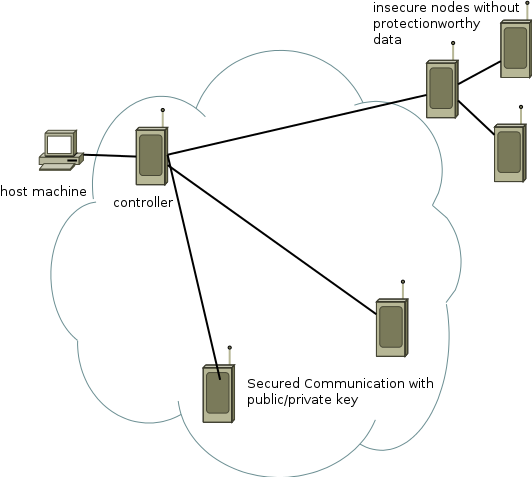
\includegraphics[width=0.6\textwidth]{pic/pkcs11.png}%
   \caption{Former idea with PKCS\#11 enabled communication between nodes}
   \label{pkcs11}%
\end{figure}


\textsc{PKCS\#11}\footnote{public-key cryptography standards} is a collection of standards related to cryptography, especially hardware supported.
In~\cite{PKCS_RSA} the API\footnote{Application Programming Interface} is described over a multitude of sites for the interested reader.
Software tokens are included in every current browser from the Mozilla foundation and all current operating systems(2012) support some means of 
hardware supported cryptography. However, due to licensing and security problems an open implementation is preferred.\footnote{Look at \url{http://www.opensc.org} for further information}

For encryption a public-private key setup could result in a fine-grained setup but there is still no development on the civil side.
The solution we had planned was based on a \(I^2C\) connectable reader for micro-sized smart cards. This would allow a setup where every node
would be addressable by its public key. A sophisticated setup would be possible.\footnote{The reasons for stopping our efforts is on human side. Pretty
bad but not worth mentioning it in this paper.}


\chapter{wsnserver - A practical solution}

\section{Overview on Development Setup}

A setup for development is explained in table~\ref{tab:requirements}. The most basic components are 
required for hands-on development. Main issue is a python interpreter and common libraries.\footnote{For example
CherryPy, pyserial and optionally a module for SQL-bindings in Python.}

Figure~\ref{setupic} shows the last version of the used development system. The keyboard and monitor on the host machine
is just used to monitor debug output and use the included \textsl{interactive} mode on the \textsc{WSN}.\footnote{So you can 
type in commands meant for nodes on the host machine instead of using the RESTful http-access}

\ref{nodepic} and \ref{hostpic} show the expected results after a clean startup. The controller identifies itself with a
self-chosen name and exchanges basic data for database population.
 

\begin{table}[h] 
\centering 
\begin{tabular}{|l||l|} 
General Component & Specific Component\\ 
\hline 
i86 host machine & 300MHz, 512MB\\ 
host OS & Debian stable(Squeeze) \\ 
Python Interpreter & Python 2.7 with pyserial \\ 
Database & MySQL\footnote{A local SQLite version with reduced functionality has no additional requirements} \\ 
1 Wireless Sensor Node as Controller & Renesas ZMD28-BRD \\
n Wireless Sensor Node as Client & Renesas ZMD28-BRD \\ 
\end{tabular} 
\caption{ Table of Requirements} 
\label{tab:requirements} 
\end{table}


\begin{figure}[H]
   \centering
   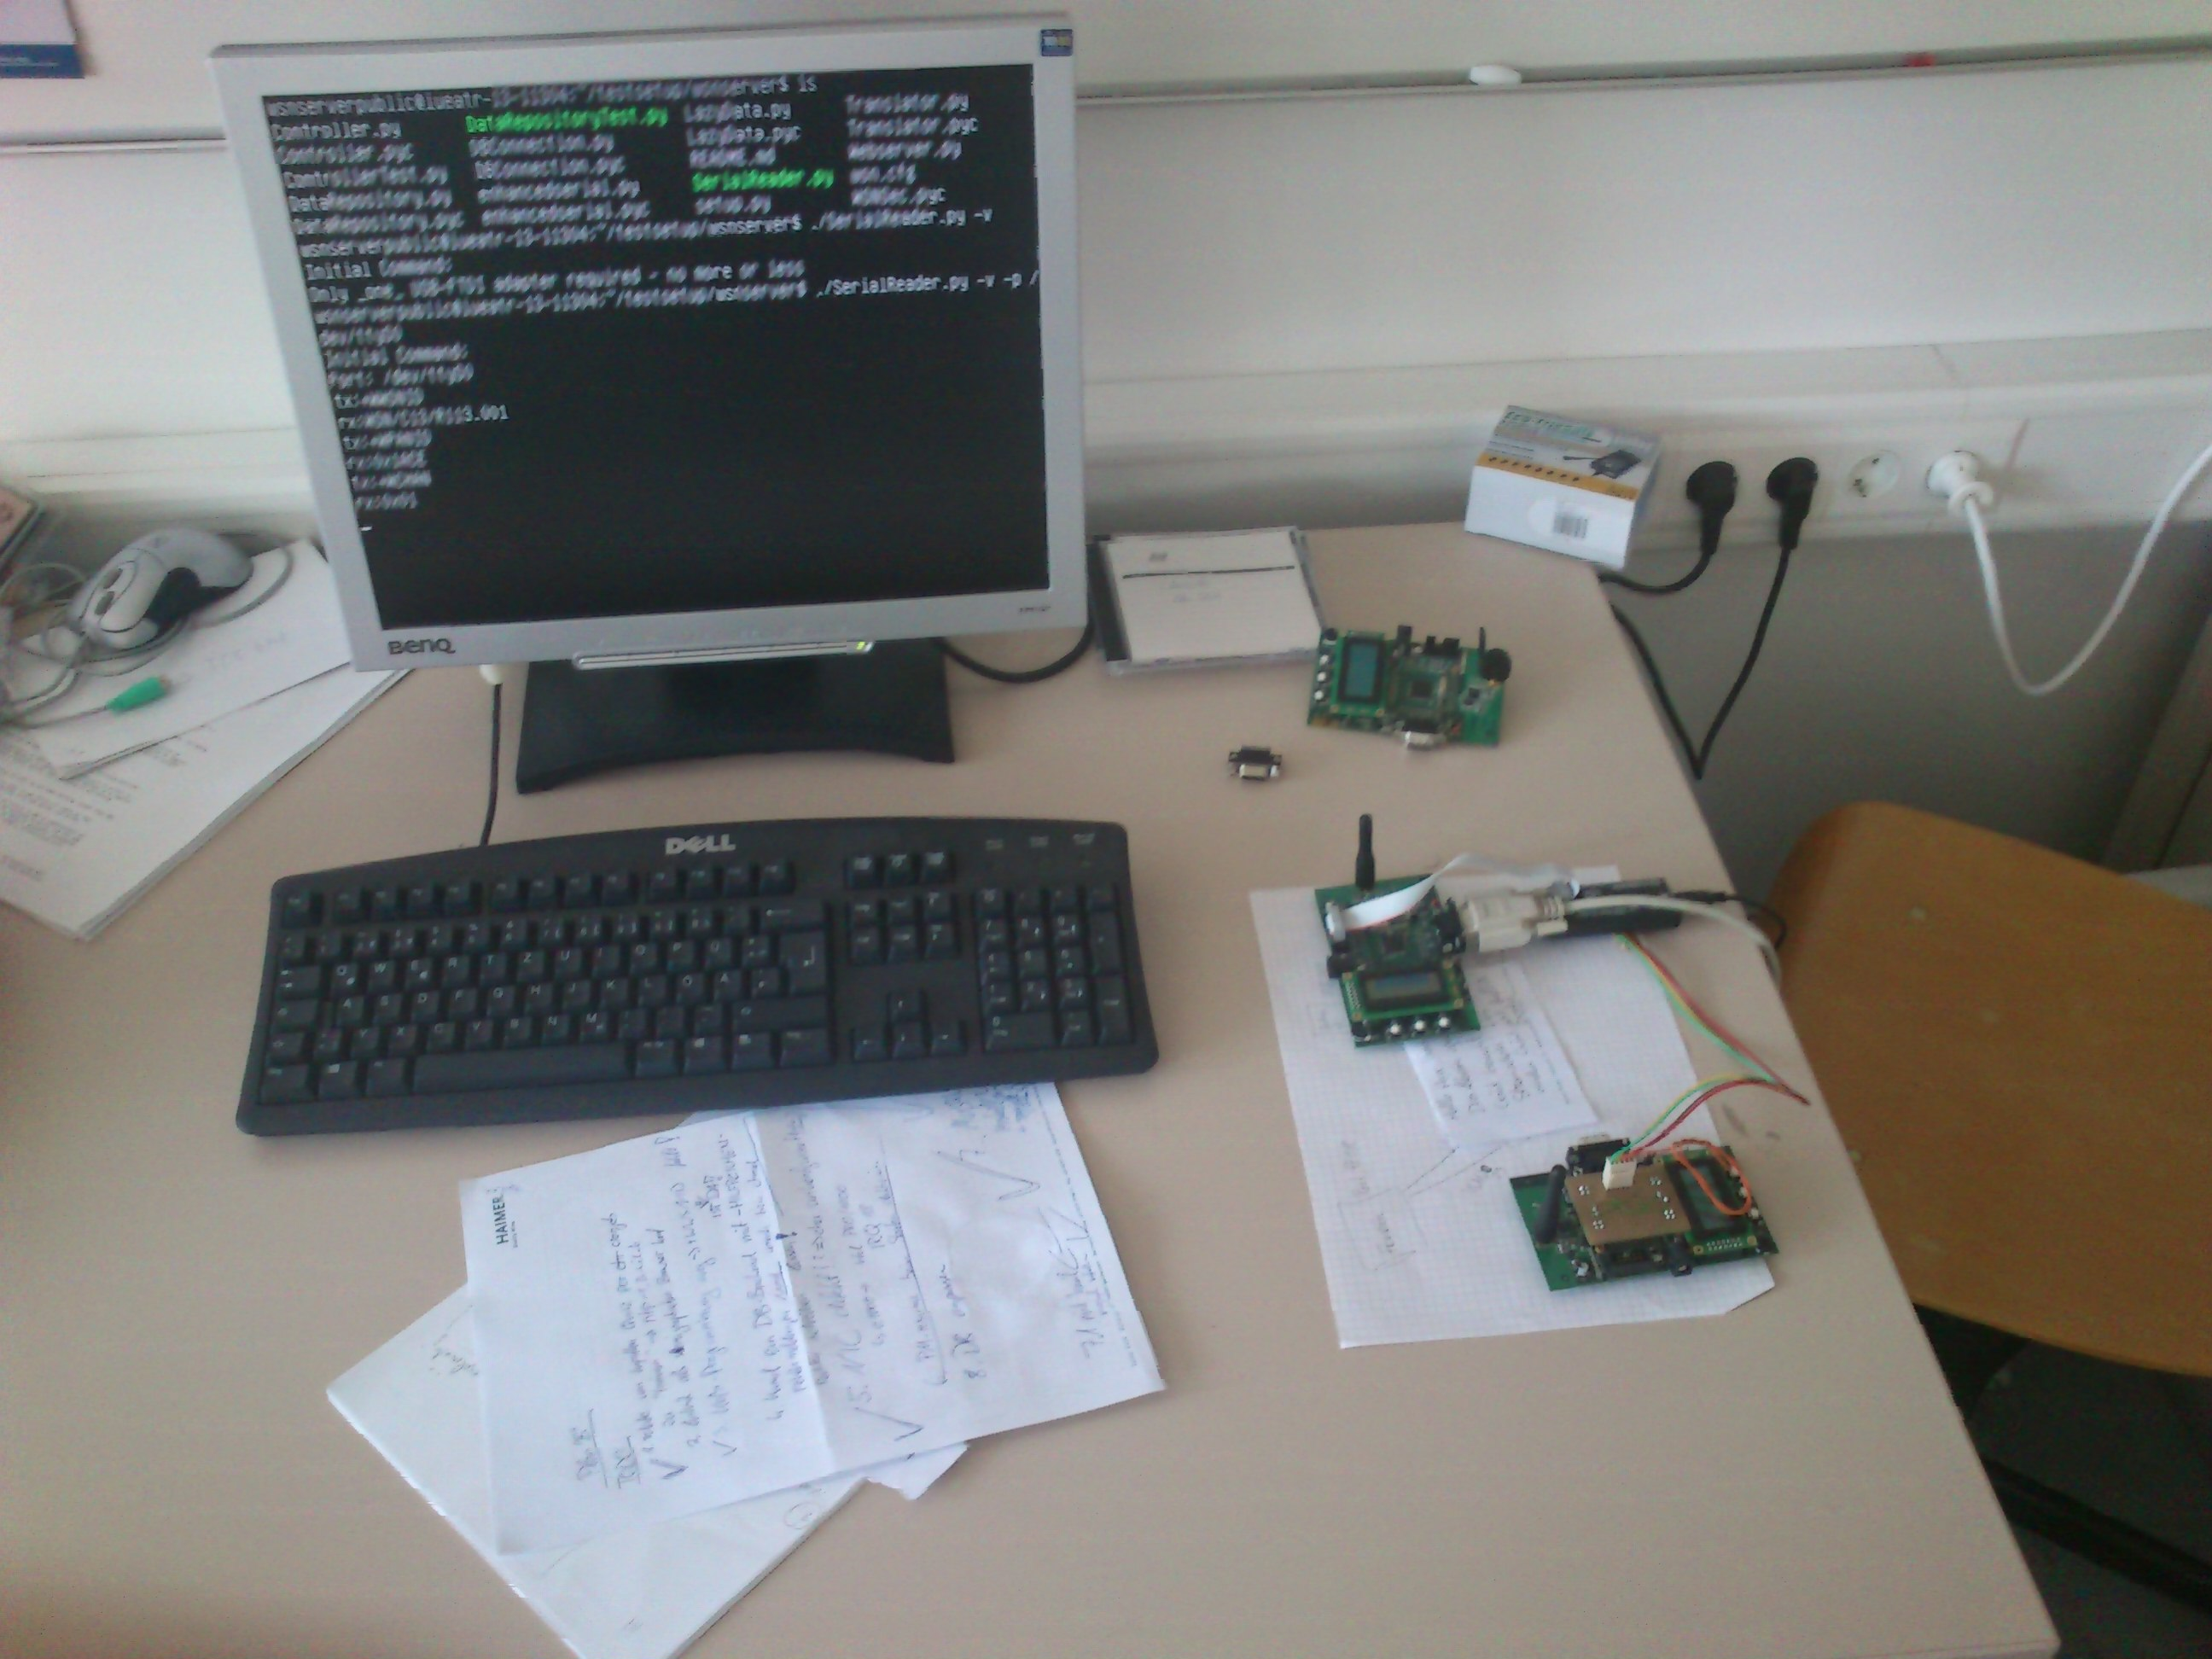
\includegraphics[width=0.8\textwidth]{pic/whole_setup.jpg}%
   \caption{Glimpse on the development setup}
   \label{setupic}%
\end{figure}

A disc image will be distributed along this document but a download is also available.\footnote{\url{XXXXXXXXXXXXXX} and use 
\url{http://clonezilla.org} as your tool of restoration.}

Look up on chapter~\ref{sec:install} on page~\pageref{sec:install} for detailed installation instructions without using the disc image.

For general x86-machine there are not specific demands 

\begin{figure}[H]
   \centering
   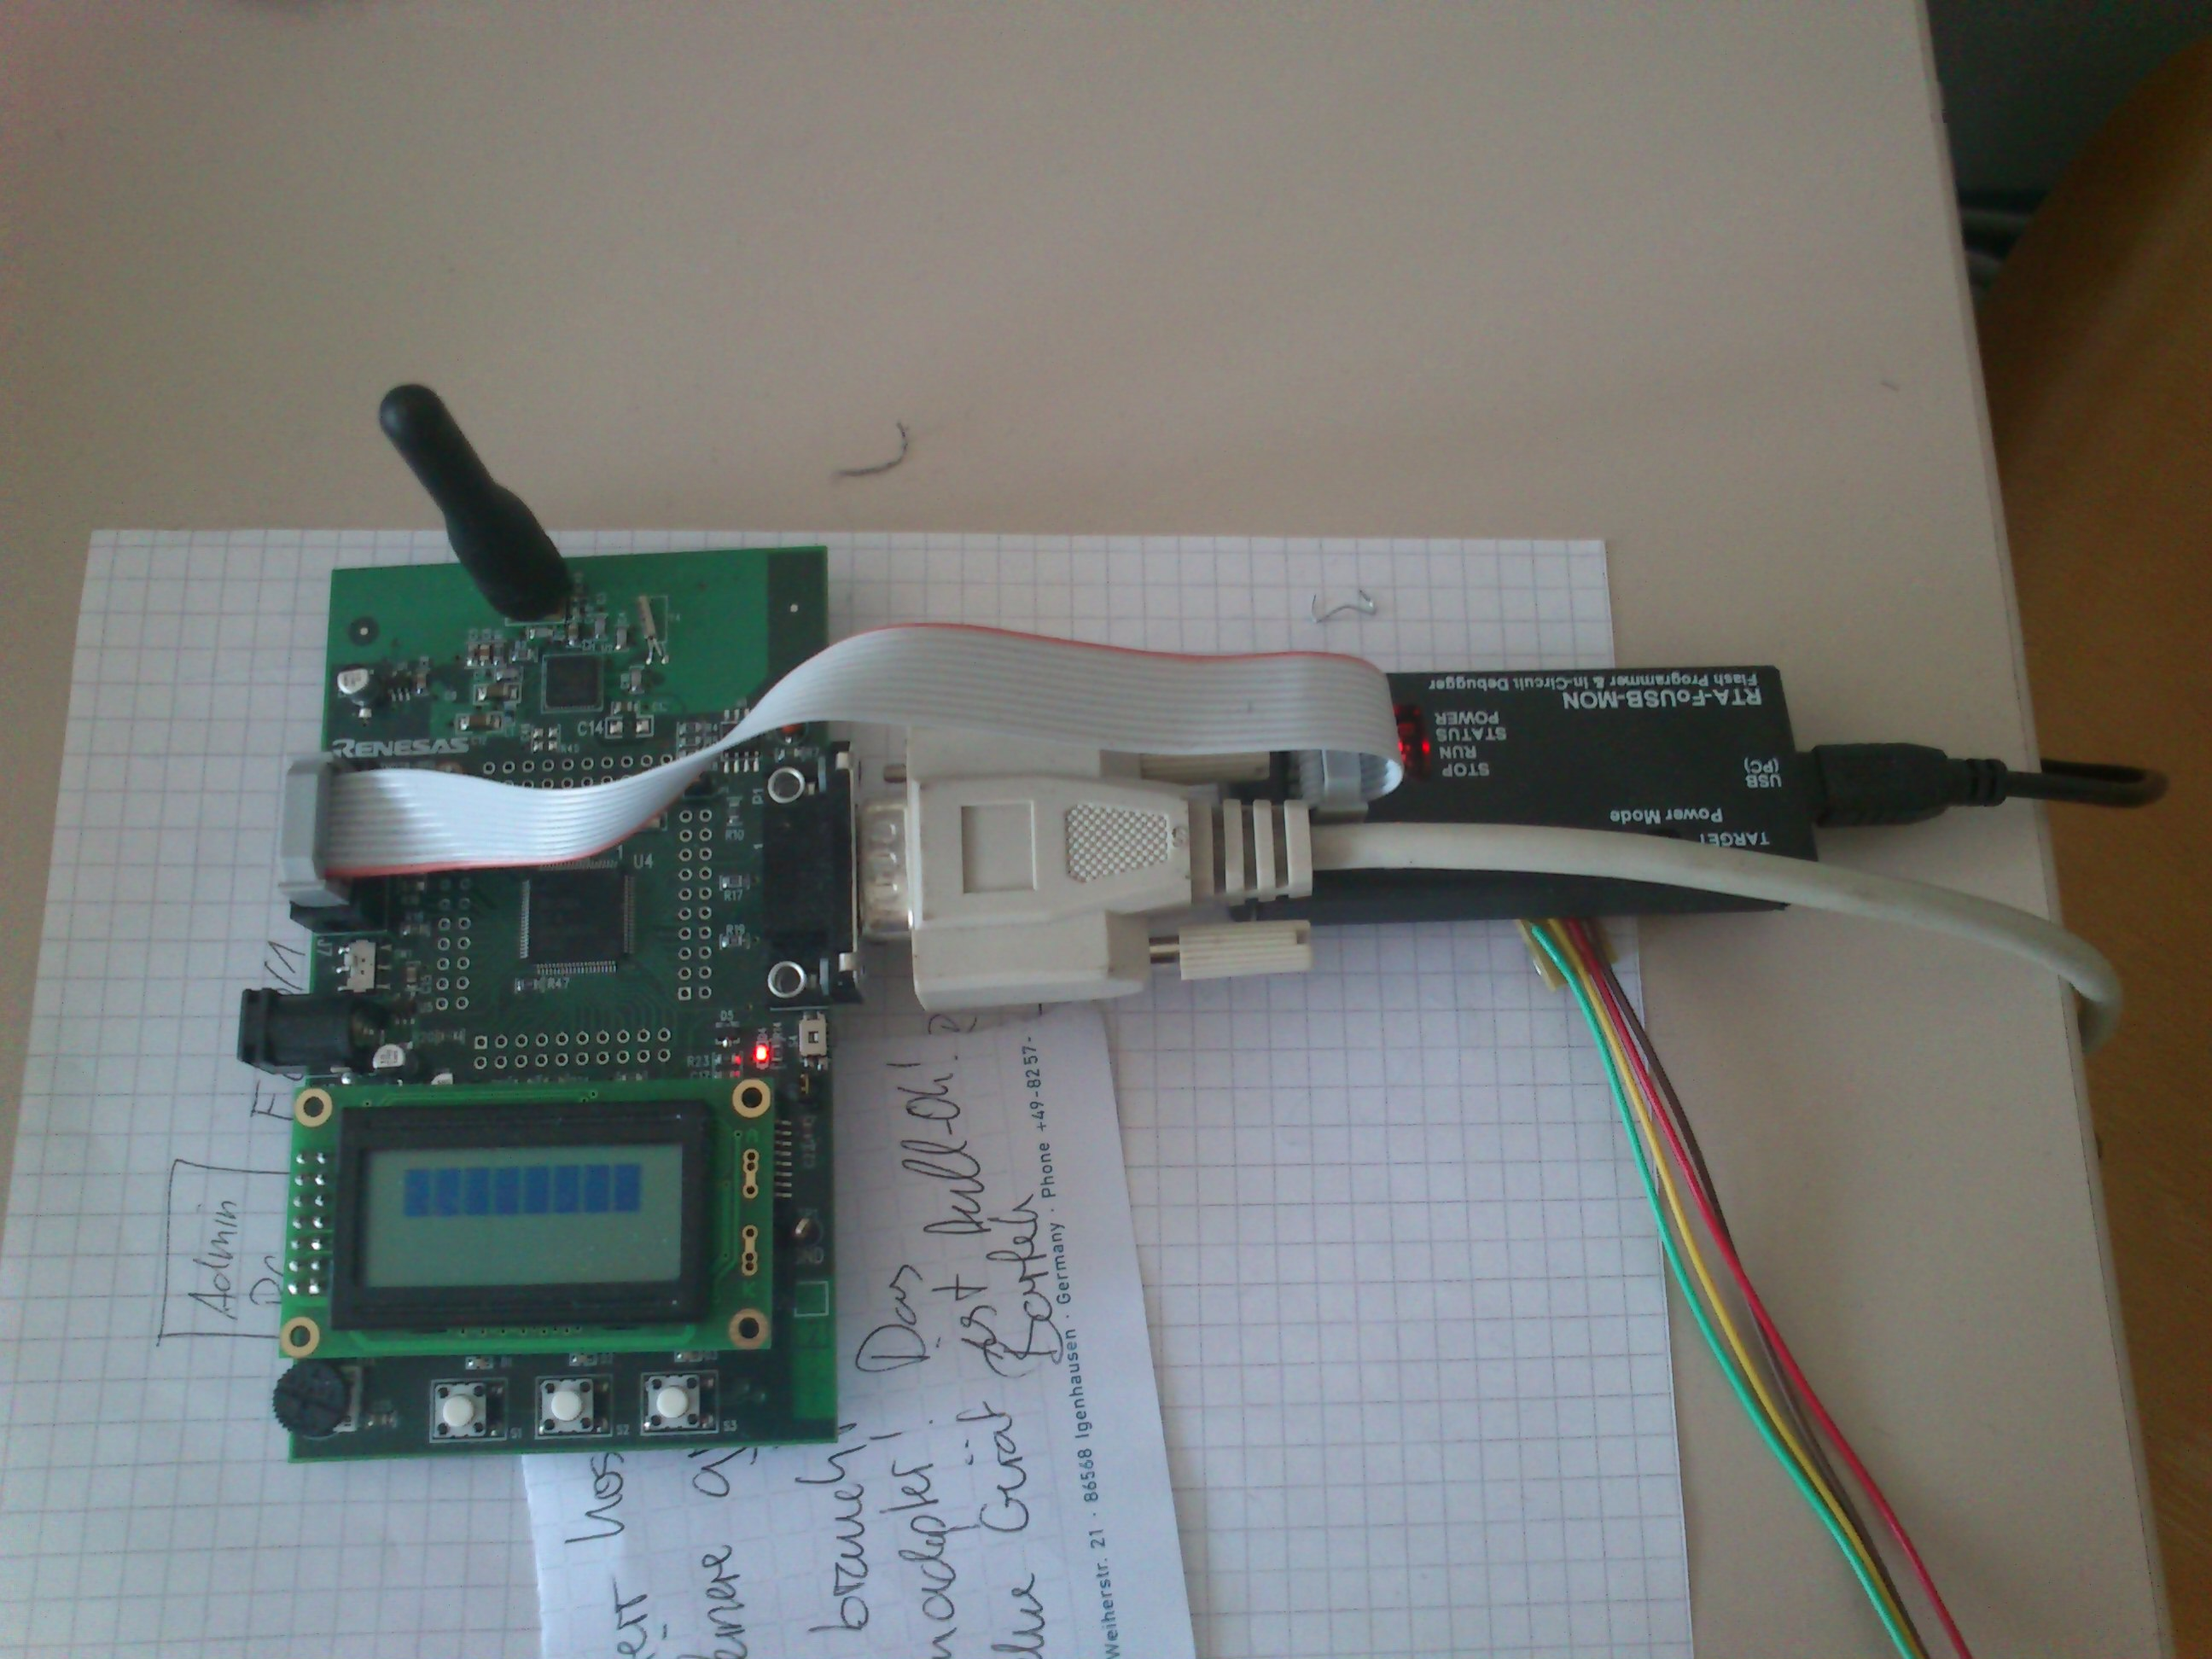
\includegraphics[width=0.8\textwidth]{pic/controller.jpg}%
   \caption{Renesas Node with Custom Programming and Serial Connector}
   \label{fig:nodepic}%
\end{figure}

For the setup we tried to not distract ourselves from the goal so we tested with just one client. The final version is not restricted
to any finite number by the translator but only by available hardware and lower protocol stack's requirements.

\begin{figure}[H]
   \centering
   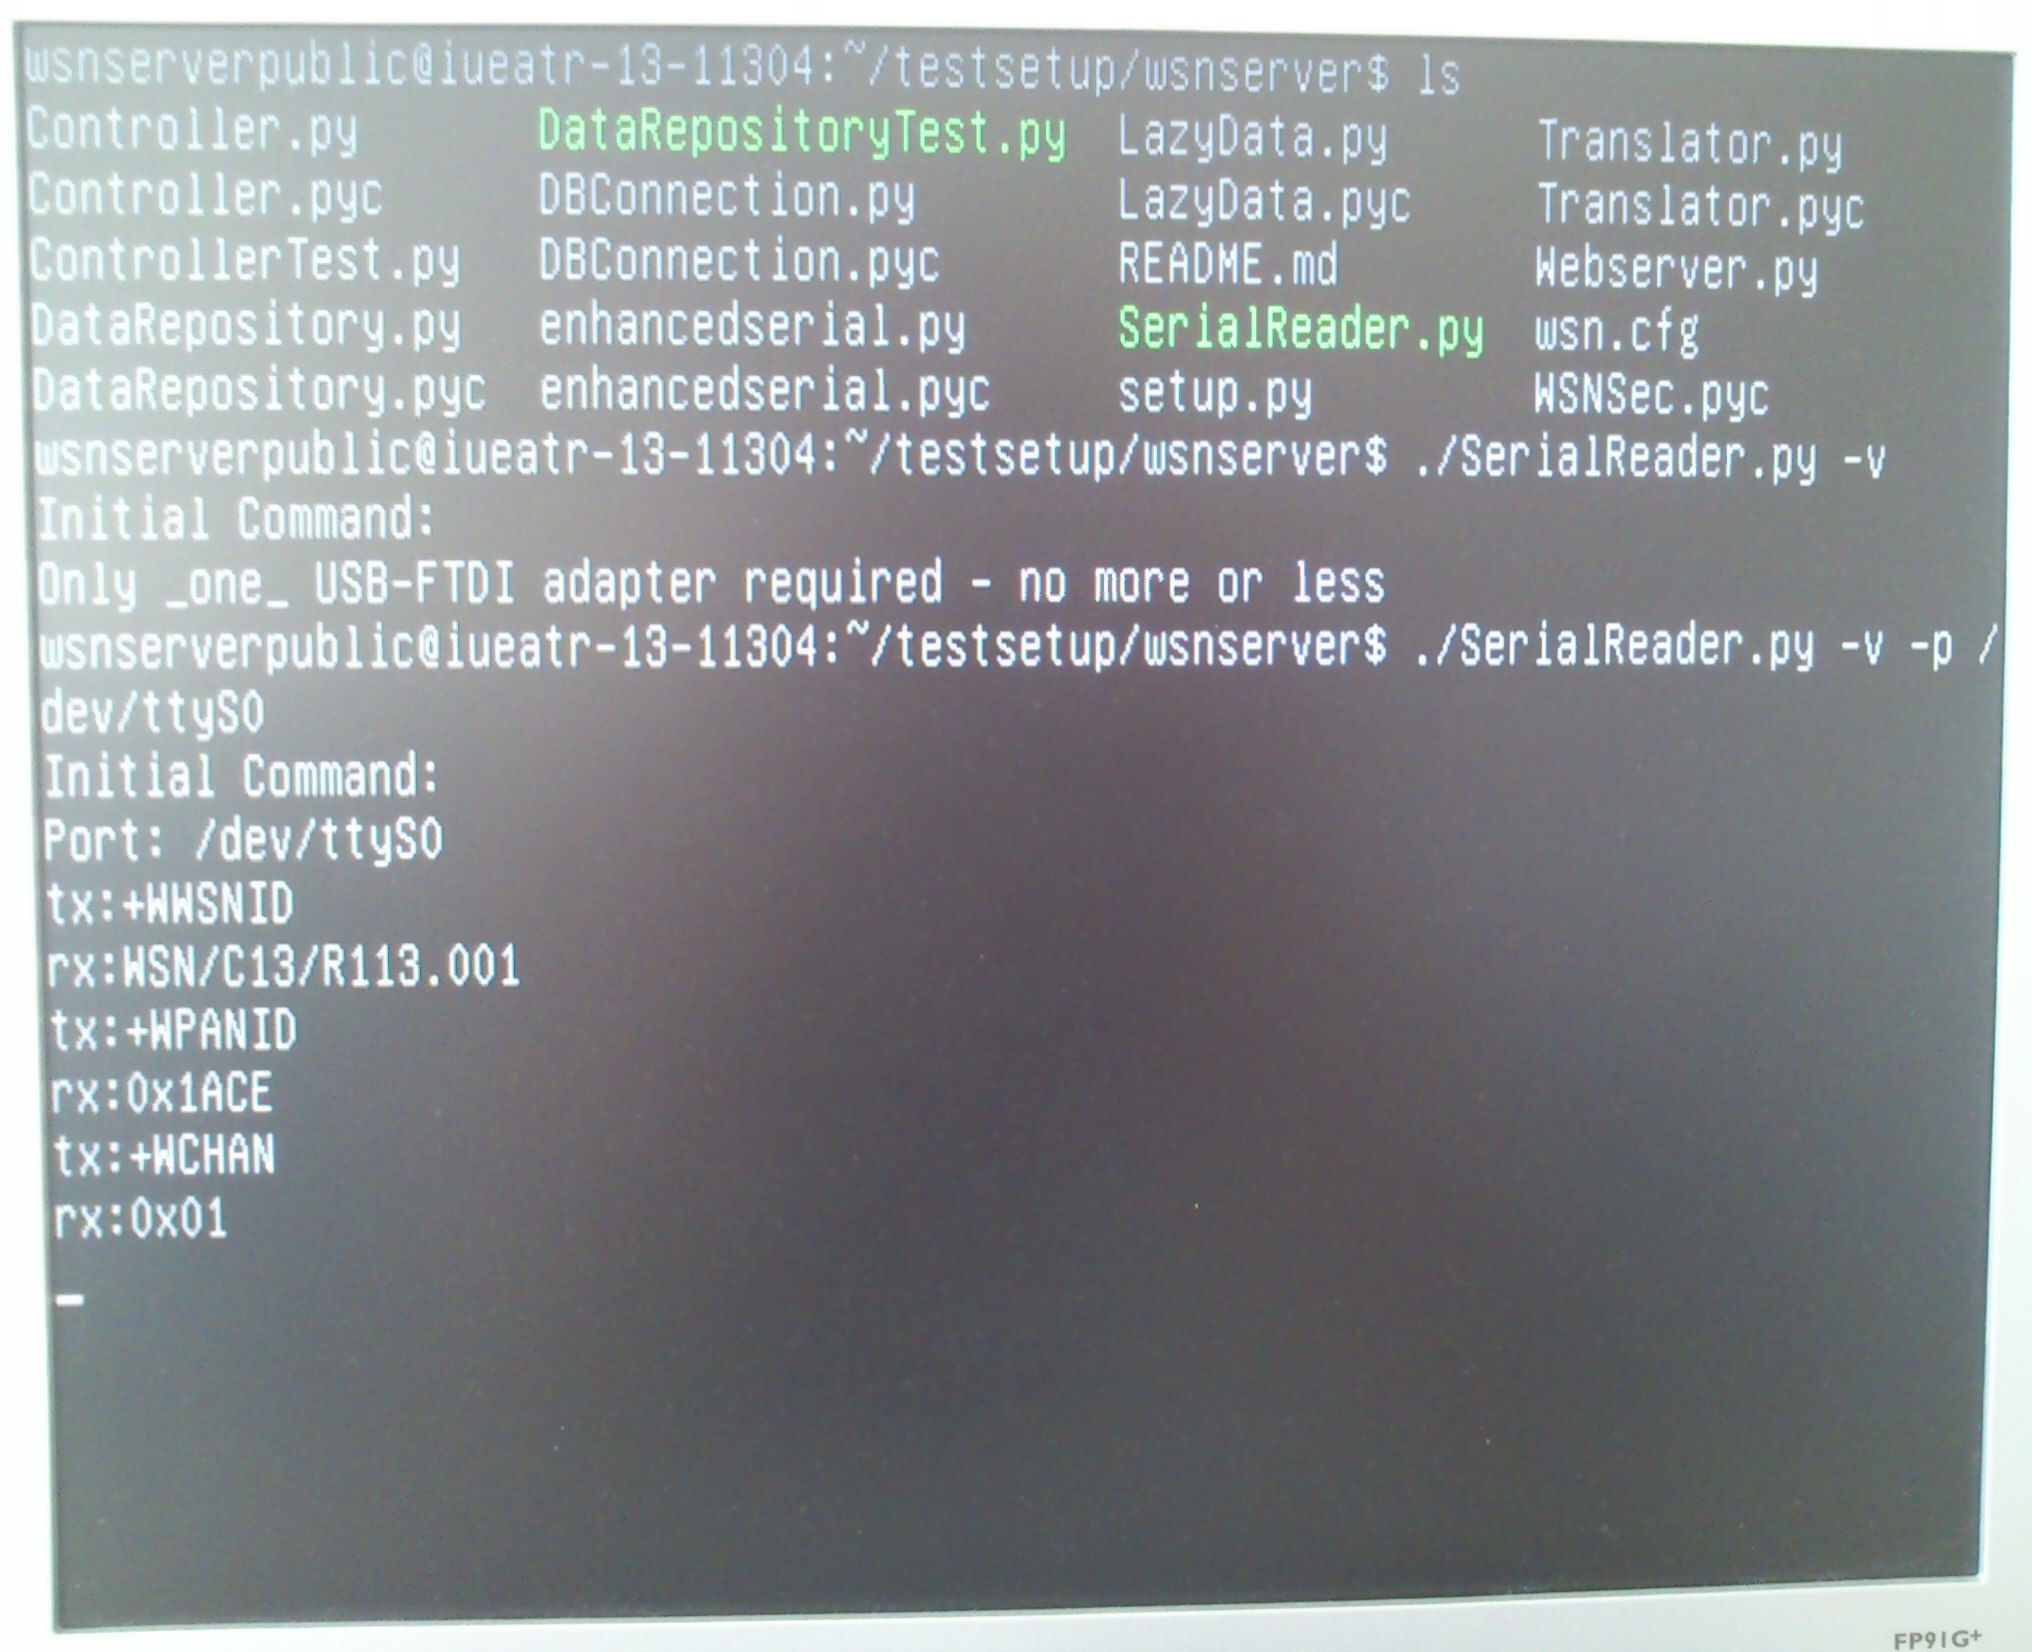
\includegraphics[width=0.8\textwidth]{pic/host_machine.jpg}%
   \caption{Console Output on Host Machine}
   \label{fig:hostpic}%
\end{figure}

Figure~\ref{fig:hostpic} shows the state of the middleware after initialisation. On default a USB-FTDI adaptor is used to enable serial over USB.
In this test we used plain RS232 connections for accessing the controlling node. The parameters of the hardware part called \textit{SerialReader.py}
are very extensive so use the code or see a console output by using the standard \textit{--help} parameter upon start.

The next step is to identify all available nodes. Firstly, the controller gets the command \textit{+WWSNID} to report example identification numbers.
Our example shows our room number in our college where the node was resting on the table as shown in picture~\ref{fig:nodepic}. It is possible 
to use whatever means of identification but it should be unique due to its importance as database key. Every node has its own 
entry and is addressable if the lower stack on the controller/router enables it.

Furthermore visible is the ZigBee identifier for \textsc{Pan Id} and \textsc{Channel Id}. Every device has its own identifier in the ZigBee specification
but it is not required on the middleware's side. Some example output is reported by the node as you can see on the screenshot.\footnote{The screenshot
    is the debug output from the host machine. This is not the default as the host could possibly run headless. Be aware that ZigBee devices may influence
other nodes which are not part of your project. We experienced this quirk and had a lot of fun to find out why.}

\newpage
\section{The development method}

For development there have been used different approaches. Most of this project has been developed by the use of agile methods, 
what means that a feature was implemented and then tested. If it worked properly, it has been committed to a central repository. 
Critical parts like the \textit{Controller} and the \textit{DataRepository} classes have been developed by using the test-driven-development, 
where first tests have been written and afterwards the corresponding methods. This last development technique had their advantages and made 
the expansion of the \textit{DataRepository} class with a second database layer - MySQL - much easier and faster: each test case 
created for the first database layer - SQLite - had also to work with the newly implemented layer for MySQL.

The approach for the hardware backend was similar but more experimental due to the serial nature of communication between node and host machine. Only
few tests were used as there were different approaches in the life-cycle of this project: a thread-based approach was not found optimal because 
of error in the \textit{pySerial} module and hardware design flaws for threading. A buffer was inserted instead which will cache a limited amount of commands which
will be sent on the next cycle. The cycles were parted between reading and writing.

\section{Desgin concept}
[HIER KOMMT NOCH EIN UML DIAGRAMM REIN, WIE WIR UNS DAS AM ANFANG VORGESTELLT HABEN  + BEHAVIORAL DIAGRAMS (Sequensdiagram + USE CASE)- KAMILLES AUFGABE]

\newpage
\section{The datamodel - database}
The datamodel is being handled by 

\subsection{Data table}
\begin{figure}[H]
	\centering
	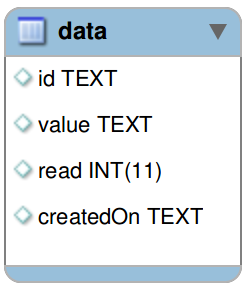
\includegraphics[width=0.3\textwidth]{pic/DatamodelData.png}%
    \caption{Representation of the data-model in the database}
    \label{DatamodelDatapic}%
\end{figure}

The data table stores the data received from the \textit{SerialReader} in the database.

\begin{description}
	\item[id] contains the wsn-id, for example \textit{wsn01}
	\item[value] this field can be used universal as it can store every data type. In the test setup was a temperature value stored.
	\item[read] represents if a stored value has been already read by a external application or if this data is still "\textit{fresh}".
	\item[createdOn] contains the timestamp to make it easier to sort and analyse data afterwards.
\end{description}

\newpage
\subsection{Device table}
\begin{figure}[H]
	\centering
	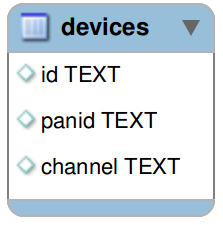
\includegraphics[width=0.3\textwidth]{pic/DatamodelDevices.png}%
    \caption{Representation of the device-model in the database}
    \label{DatamodelDevicespic}%
\end{figure}

The device table stores the devices connected to the system. The idea behind this table was to provide wsn-ids of the connected devices to external applications. Connecting this functionality with the \textit{Webserver} opens new possibilities and services like the implemented \textit{sendCMD} method in the \textit{Webserver} class. By knowing the wsn-ids it enables the application to create new commands and store them in the database.

\begin{description}
	\item[id] contains the wsn-id, for example \textit{wsn01}.
	\item[panid] contains the panid.
	\item[channel] stores the channel, on which the wsn is communicating.
\end{description}

\newpage
\subsection{Command table}
\begin{figure}[H]
	\centering
	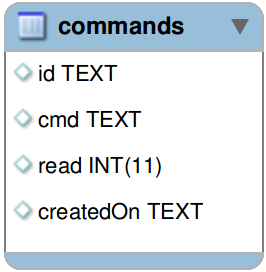
\includegraphics[width=0.3\textwidth]{pic/DatamodelCMD.png}%
    \caption{Representation of the command-model in the database}
    \label{DatamodelCMDpic}%
\end{figure}

As already addressed in the description of the \textit{device} table the \textit{command} table stores commands for wireless sensor nodes. This table is used as buffer between the application, which send this command, and the wireless sensor node, which will execute the command.

\begin{description}
	\item[id] contains the wsn-id, for example \textit{wsn01}.
	\item[cmd] contains the command, for example \textit{GetID}.
	\item[read] represents if a stored command has been already executed by the \textit{SerialReader}.
	\item[createdOn] contains the timestamp. It is needed for the execution of the \underline{newest} command.
\end{description}

\newpage
\section{Class diagrams}
\subsection{Setup.py installation script}
The first step in setting up the middle-ware is to run the \textit{Setup.py} installation script by using \textit{python Setup.py --option}. The goal of the \textit{Setup.py} is to configure the database connection and also to create the needed tables in the database. A configuration file named \textit{wsn.cfg} is being created, which stores the type and the connection settings. In case of the creation of a \textit{SQLite} database, no authentication credentials are needed.

Furthermore the \textit{Setup.py} allows the cleaning of the tables by using the \textit{--rmDev},  \textit{--rmData} and \textit{--rmCMD} and also to change the database type form for example \textit{SQLite} to \textit{MySQL}.

\begin{figure}[H]
	\centering
	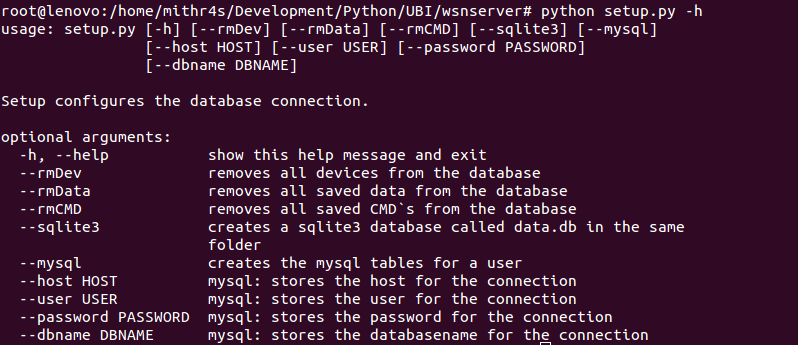
\includegraphics[width=1.0\textwidth]{pic/Setuppy.png}%
    \caption{The help page of the Setup.py script.}
    \label{Setuppypic}%
\end{figure}

\newpage
\subsection{The Controller class}
\begin{figure}[H]
   \centering
   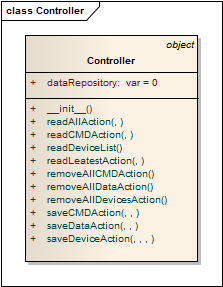
\includegraphics[width=0.5\textwidth]{pic/Controller.png}%
   \caption{The Controller class}
   \label{Controllerpic}%
\end{figure}

The \textit{Controller} class is the central part of this project. It corresponds to the controller part of the Model-View-Controller design pattern.

Like in any other MVC applications the controller receives and handles input and requests of the user and also of any other external modules. 
It validates the input and decides what to do with the data passed to the controller, 
for example if the controller should save it to the model or retrieve some data from the repository and return it as response.

Applied to this project the \textit{Controller} class receives requests from the web server to retrieve stored data for a 
WSN and also to save commands for a WSN in the database, which is used as a queue. The second actor of this class is the 
\textit{SerialReader} class, which also accesses the controller to save its identification credentials, 
to pass its read sensor data to the controller for saving and to retrieve new commands from the queue.

The last possible user is the setup script, which accesses the controller for maintenance tasks, like removing all data from the data repository.



\newpage
\subsection{The ControllerTest class}
\begin{figure}[H]
   \centering
   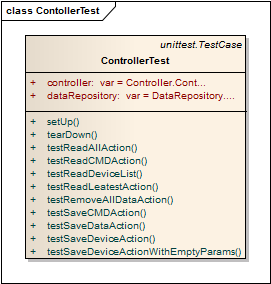
\includegraphics[width=0.5\textwidth]{pic/ControllerTest.png}%
   \caption{ControllerTest class, unittest for the Controller class}
   \label{ControllerTestpic}%
\end{figure}

This unittest was written to test the \textit{Controller} class and their functionality. 

The \textit{setUp()} method creates fixtures, which will be stored in the database, before each test case will be run. This ensures that all "retrieving"-methods have something to read and all "remove"-methods have something to delete. At the end of each test case the expected and the actual values will be compared. 

After each testrun the database will be cleared by the \textit{tearDown()} method. 

\newpage
\subsection{DataRepository class}
\begin{figure}[H]
   \centering
   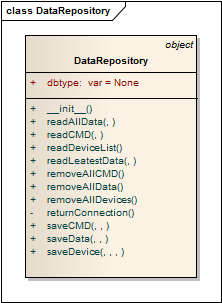
\includegraphics[width=0.5\textwidth]{pic/DataRepository.png}%
   \caption{DataRepository class, which handles the model}
   \label{DataRepositorypic}%
\end{figure}

The \textit{DataRepository} class is the main model class of this project. 
Their goal is to store and retrieve information and data from the database. 
Nearly all methods contain SQL instructions, 
which will be executed by the use of an \textit{DBConnection} object, which again contains an actual database connection.

In the first implementation the methods have been developed to run with SQLite so no other database system was needed. After running a few stresstests - by storing very much data in a very short time in the database - the database crashed. Therefore a second layer - MySQL - was developed to ensure proper function under high database usage.

\newpage
\subsection{DataRepositoryTest class}
\begin{figure}[H]
   \centering
   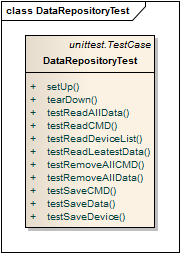
\includegraphics[width=0.5\textwidth]{pic/DataRepositoryTest.png}%
   \caption{DataRepositoryTest class, unit test for the DataRepository class}
   \label{DataRepositoryTestpic}%
\end{figure}

Equivalent to the \textit{Controller} class the \textit{DataRepository} class also possesses a test class.

The testing of the \textit{DataRepository} class was very crucial, because it was very important to ensure the proper function of the methods implemented in the \textit{DataRepository}. A small error could later cause a discrepancy when analysing the data retrieved from the database. 
The tests have been developed to be executed for the \textit{DataRepository} in its first version with SQLite, but the same tests also accelerated the development of the MySQL-layer, because every test, which has been developed to run with SQLite, had also to work identically with the MySQL-implementation.

\newpage
\subsection{DBConnection class}
\begin{figure}[H]
   \centering
   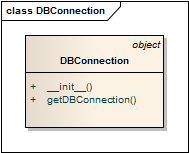
\includegraphics[width=0.5\textwidth]{pic/DBConnection.png}%
   \caption{DBConnection class, a database layer}
   \label{DBConnectionpic}%
\end{figure}

The sole purpose of the \textit{DBConnection} class is to return an open database connection to the caller. 
This is achieved by loading the configuration file and read out the settings, so the \textit{DBConnection} 
class can decide which kind of database connection it will return to gridlabels=the calling method as response.

\newpage
\subsection{EnhancedSerial class}
\begin{figure}[H]
   \centering
   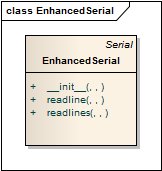
\includegraphics[width=0.5\textwidth]{pic/EnhancedSerial.png}%
   \caption{EnhancedSerial reader class}
   \label{EnhancedSerialpic}%
\end{figure}

\textit{EnhancedSerial} is a part of \url{http://pyserial.sf.net}{pyserial}  written by \href{mailto:cliechti@gmx.net}{C. Liechti} in 2002.
It is a huge improvement in comparison to the default serial line communication class. For details please look into the code.


\newpage
\subsection{LazyData class}
\begin{figure}[H]
   \centering
   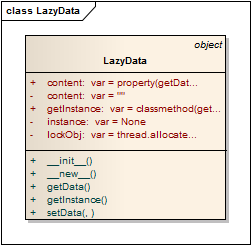
\includegraphics[width=0.5\textwidth]{pic/LazyData.png}%
   \caption{LazyData class}
   \label{LazyDatapic}%
\end{figure}

\textit{LazyData} is a singleton based on the work of Alan Felice. Mainly it serves as a data buffer for the serial output from the host to the node. 
As mentioned by~\cite{GammaHelmJohnsonVlissides199711} the singleton only allows one instance which is accessible throughout every object. It was
heavily modified by us to enable the usage for the serial reader module.

\newpage
\subsection{Translator class}
\begin{figure}[H]
   \centering
   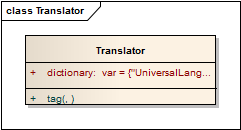
\includegraphics[width=0.5\textwidth]{pic/Translator.png}%
   \caption{Translator class}
   \label{Translatorpic}%
\end{figure}

The translation abstract class is the heart of the middleware. It enables the transition between the various language by providing a basis for further 
abstraction.

\subsubsection{MedusaTranslator class}
\begin{figure}[H]
   \centering
   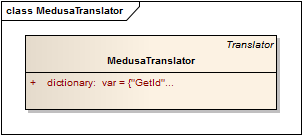
\includegraphics[width=0.5\textwidth]{pic/MedusaTranslator.png}%
   \caption{MedusaTranslator class}
   \label{MedusaTranslatorpic}%
\end{figure}

The Medusa is a node system with a lot of sonar-like \textit{heads} which are mainly used in localisation.\cite{Dispert}
This is just a symbolic help to insert also this very special node in the translation system.

\begin{figure}[H]
   \centering
   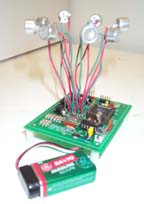
\includegraphics{pic/medusa.jpg}%
   \caption{A first generation Medusa. Image source: \url{nesl.ee.ucla.edu}}
   \label{Medusapic}%
\end{figure}


\subsubsection{RenesasTranslator class}
\begin{figure}[H]
   \centering
   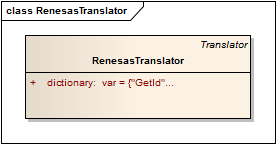
\includegraphics[width=0.5\textwidth]{pic/RenesasTranslator.png}%
   \caption{RenesasTranslator class, dictionary class for Renesas}
   \label{RenesasTranslatorpic}%
\end{figure}

As the Renesas ZMD28-BRD is used as our main development board we included a full class for temperature sensing. It is a very 
basic hardware programming on the node to not complicate the whole project. It was provided by the laboratory assistant Stephan Ko\ss.

The class itself is mainly a dictionary which is used for the translation process.

\newpage
\subsection{SerialReader class}
\begin{figure}[H]
   \centering
   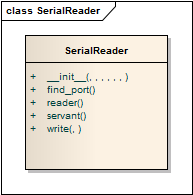
\includegraphics[width=0.5\textwidth]{pic/SerialReader.png}%
   \caption{SerialReader class, main class for reading data from serial port}
   \label{SerialReaderpic}%
\end{figure}

\textit{SerialReader} is used for the hardware part. It is highly configurable through parameters and even more through code. As the
serial RS232 connector utilizes a big amount of different configuration parameters a possible adaptor will surely have to look inside the
programming. It is the main component which must be started.\footnote{Also the database is important if you don't want to rely on sqlite.}

\newpage
\subsection{Webserver class}
\begin{figure}[H]
   \centering
   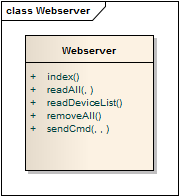
\includegraphics[width=0.5\textwidth]{pic/Webserver.png}%
   \caption{Webserver class, containing the web server}
   \label{web serverpic}%
\end{figure}

The \textit{Webserver} class can be seen as the \textit{View} part of the MVC pattern, as it allows and restricts the access and the requests of a user to this specified methods.

The class uses the CherryPy web server framework.\footnote{The CherryPy web server is a open source project hosted on \url{http://www.cherrypy.org/}} A standalone web server written completely in Python. The advantage of this fact is that the dependency of project is reduced to Python instead of the use of a big and resource hungry web server like Apache2. Also the easy and fast development of methods/pages which comes with the framework.

For demonstration of the simplicity of CherryPy an extract of the \textit{Webserver} class is presented. As it can be seen, it is already enough to define a method to receive a functional site. 
\begin{lstlisting}[language=Python]
import Controller
import cherrypy
from cherrypy import expose

class web server:
    @expose
    def index(self):
        return "WSN-Server is up and running"
       
\end{lstlisting}

To see if this method works, the user has to call \url{http://localhost:8080/index} and will receive the status of the web server.

Some of the methods defined in this class need parameters to retrive or save data for a specific \textit{wsn-id}. To provide an example the \textit{readAll} method has been choosen. Its purpose is to retrieve all data for a specific \textit{wsn-id}.
\begin{lstlisting}[language=Python]
@expose
    def readAll(self, id):
        controller = Controller.Controller()
        string = format(controller.readAllAction(id))
        return string
\end{lstlisting}
It will be assumed that in the \textit{data} table data for a WSN device with the id \textit{wsn01} is stored. To get this data the user or application has to call the following url with the id as parameter: \textit{http://localhost:8080/readAll?id=wsn01}.
It is important to use the parameters specified in the method as url parameters, else the web server will not recognize it and won't retrieve the data. 

\newpage
\section{Custom Installation}
\label{sec:install}

Custom installation is only required when not using the provided disc image.

\begin{enumerate}
    \item Install a Linux of your chosen flavour. Preferably use Debian.
    \item Install git\footnote{\textit{apt-get install git}}
    \item Download and install cherrypy\footnote{\url{http://www.cherrypy.org/wiki/CherryPyDownload} or on Debian \textit{apt-get install python-cherrypy}}
    \item Run \textit{python setup.py --sqlite} to create and configure the SQLite database. For further information or help run \textit{python setup.py -h}, which explains the usage of the commandline script.\footnote{This step is only required if you do not use the MySQL backend}
    \item \textit{Optionally:} Install a MySQL server and proper SQL bindings for increased functionality\footnote{\textit{apt-get install mysql-server mysql-client libmysqlclient15-dev python-mysqldb}}
\end{enumerate}

The last step is to use a proper user-account\footnote{root not recommended but put the user in the appropriate group for accessing serial connection} and
get the most recent development version with git.\footnote{\textit{git clone git@github.com:Phialo/wsnserver.git}}

Finally, you change directory to the project and run \textit{python SerialReader.py -h} to see available options.

If there is a need to make all the gathered data and informations available for further use, the \textit{web server} can be started by running \textit{python Webserver.py}. This will automatically start the 
\textit{web server} and make all implemented methods immediately ready for use. To see which commands respectively methods are available, the user should take a look at the description of the \textit{Webserver} class.


\chapter{Conclusion}

The middleware presented in this paper is a first step of providing a modular, basic system for the development and control of wireless sensor networks, adjustable to the needs of the environment.

The created wireless sensor network server fulfils the needs of a middleware, which supports the implementation of different node protocols and various kind of sensor nodes. 

The separation of the middleware into the \textit{Model-View-Controller} layers makes the system very modular and the implementation of new communication protocols easier and faster. Developers can use the already implemented solution for the \textit{Renesas} node as aid and template for new modules and it is their option to specify the location of the connected device, like USB or the serial port. 

Furthermore the middleware contains a fully functional web server with a RESTful API for communicating with the server. Developers can customize the web server and the interface to their needs. 






%\begin{figure}[H]
%	\centering
%	\includegraphics[width=0.6\textwidth]{http.png}%
%	\caption{HTTP-Kommunikation zwischen Server und Client}
%	\label{http}%
%\end{figure}
%\footnote{L�sungsarchitekturen wie RESTful Web Services wie in der Dissertation von 
%Fielding in \cite{Fielding99softwarearchitectural} beschrieben verlagern die Identifizierung eines Benutzers und den Transport von Informationen �ber 

%\begin{description}
%\item[GET] Eine bestimmte Resource wird vom Server abgefragt. Dies kann ein statisches Dokument oder ein serverseitiges Script sein. GET-Aufrufe m�ssen in ihrer Auswirkung idempotent sein, das hei�t
%ein mehrmaliger Aufruf mit Hilfe eines GET-Requests soll die selbe Auswirkung haben wie ein einzelner GET-Request.\cite{rfc2616}\footnote{Wenn beispielsweise ein GET-Aufruf einen Einkaufsvorgang mit Bezahlung bewirken soll, muss nach 
%wiederholten des GETs kein neuer Artikel eingekauft oder Abbuchvorgang durchgef�hrt werden.} 
%\item[POST] Daten des Clients werden zur Verarbeitung an den Server geschickt. Es sind die selben 
%Header-Variablen m�glich wie im GET. Deshalb kann durch die Verwendung von Cookies hier eine Verkn�pfung zu 
%vorhergehenden GET-Aufrufen hergestellt werden.
%\item[HEAD] Eine Resource wird vom Server abgefragt aber es sollen nur die Kopfdaten einer gesamten HTTP-Verbindung als Response zur�ckgeliefert
%werden. Damit kann das Datenaufkommen verringert werden, falls nur der Antwortstatus gefragt ist.
%\end{description}

%\begin{itemize}
%\item Authentifizierung von Server und Client
%\item End-zu-End Verschl�sselung einer HTTP-Verbindung
%\item Integrit�tspr�fungen
%\end{itemize}

%daf�r die \texttt{javax.net.ssl} Klasse zur Verf�gung. Leider wird die Sessionverwaltung nicht unter anderen Plattformen 

%mit der Einbindung der PKCS-Spezifikation, die in Kapitel \ref{sec:pkcs} n�her erl�utert wird, eine M�glichkeit
%Skriptsprachen eine \textsl{same orgin policy}\footnote{\url{https://developer.mozilla.org/En/Same_origin_policy_for_JavaScript}} umgesetzt, die

%\url{http://www.whatwg.org/specs/web-apps/current-work/complete/commands.html\#devices}}

%\(c\) umwandeln kann, muss \(s\) auch zur Entschl�sselungfunktion \(E\) genutzt werden k�nnen um den
%Klartext wiederherzustellen. Die Verschl�sselung sieht folgenderma�en aus:
%\[V_s(k)=c\] 


%\subsubsection{TEA}
%\label{sec:tea}

%\begin{quote}
%
%``What does this protocol achieve?\\
% Does this protocol need more assumptions than another one?\\
% Does this protocol do anything unnecessary that could be left out without weakening it?\\
% Does this protocol encrypt something that could be sent in clear without weakening it?'' \cite{Burrows90}
%
%\end{quote}


%\begin{lstlisting}[language=PHP]
%include "sgl_wrap.php";
%
%SglFormInit($authentCode,1,"nextFile.php");
%SglSearchLock(1);
%SglFormClose();
%
%\end{lstlisting}

%\begin{table}[!h] 
%\centering 
%\begin{tabular}{|l||l|} 
%Position & Person\\ 
%\hline Manager of Student
%Group & MG \\ 
%Document Manager/Vice Lead & BD \\ 
%Head Programmer/Database Administrator & CT \\
%Quality Assurance/Programmer & GG \\ 
%Design/Diagrams & AI \\ 
%Diagrams/Head Research & SC \\
%\end{tabular} 
%\caption{ Table of responsibilities} 
%\label{tab:responsibilities} 
%\end{table}


\nocite{*}
\bibliographystyle{acm}
\bibliography{bibwsnserver}
\listoffigures
\begingroup \let\clearpage\relax
\listoftables \endgroup
\end{document} 
